\documentclass{article}
\usepackage[a4paper, total={170mm, 257mm}]{geometry}

\usepackage{graphicx}
\graphicspath{ {./images/} }
\usepackage{float}

\usepackage{multicol}
\usepackage{hyperref}
\usepackage{tikz}
\usepackage[siunitx]{circuitikz}
\usepackage{siunitx}

\title{SQA Summer Research Write Up}
\author{Cory Aitchison}
\date{Summer 2021}

% \twocolumn
\begin{document}
\maketitle

\begin{multicols*}{2}

    \section{Introduction}

    This document aims to be a brief summary of results, and instructions for how to access data. Files are mostly located at:

    \begin{description}
        \item[Room 101] \verb`C:/Data/users/Cory`
              % \item[LGxxx] \verb`C:/Data/...`
    \end{description}

    \section{Transistor Characterisation}

    Resistance, current and voltage measurements for the MOSFET transistor in operation.

    \subsection{Equipment}

    \begin{itemize}
        \item Transistor: \verb:CE3512K2:
        \item Source: Electrode $33$
        \item Drain: Electrode $39$
        \item Gate: Electrode $40$
    \end{itemize}

    \noindent When applying voltages (drain-source, gate) it was connected such that:

    \begin{itemize}
        \item $v_{DS}$ connected with positive on the source; negative/ground on the drain
        \item $v_\mathrm{gate}$ connected with positive on the gate
        \item Ground wire from $v_\mathrm{gate}$ output is connected to the ground of $v_{DS}$. This ensures that grounding is correct for the two voltages.
    \end{itemize}

    See \autoref{fig:dcconnect} for circuit diagram.
    \begin{itemize}
        \item Connected using 2 SMUs and one variable DC Source (SMU1 - supply $v_{DS}$ and measure $I$; SMU2 - measure $v_{4-wire}$; DC Source - supply $v_\mathrm{gate}$)
        \item It is possible using just 1 SMU, 1 DC source, and 1 voltmeter
        \item Ensure that the RF cable (e.g. to the VNA) is disconnected before running current sweeps; it adds quite a lot of noise to the measured current
    \end{itemize}

    \subsection{Measurements}

    4-wire sensing measurements: Figures \ref{fig:4wirecurrentline}, \ref{fig:4wirecurrent}, \ref{fig:4wireresistance}, \ref{fig:4wirevoltage}. We see that the device can turn on (max current) and off (no current) by sweeping the gate voltage $-2$ to $0$ V.

    Some artifacts emerge due to the Yokogawa IM7651 changing range near $-1$ V.

    \section{Copenhagen Board}

    The board has DC resistance $1.2\si{\kilo\ohm}$ and $6.188\si{\kilo\ohm}$ for board \verb`#25` and \verb`#26`. This combines to a $7.388\si{\kilo\ohm}$ resistance in series with the transistor (e.g. for the source/drain).

    \section{Reflectometry}

    RF reflectometry to act as a probe for the resistance of the transistor.

    \subsection{Equipment}

    \begin{itemize}
        \item \verb`VNA4396B` used for measuring reflected power
        \item Set to \verb`Start`: $1\si{\mega\hertz}$ and \verb`Stop`: $250\si{\mega\hertz}$
        \item Measuring $A/B$ and Scale = \verb`Auto scale`
        \item Connected to $M4$ on the CPH board
    \end{itemize}

    \subsection{Measurements}

    \noindent Resonances with the transistor are observed at values as per \autoref{table:capacitances}. The large parasitic capacitance corresponding to the source electrode can be accounted for by considering that the transistor has a larger surface area than conventional quantum devices (with $C_p \sim 1\si{\pico\farad}$).

    \noindent Resonances without the transistor correspond to: $166$, $198$, $231$, and $275$ MHz.

    Simulated resonance peaks are at \autoref{fig:resonancesim} and \ref{fig:s11cs0db}. Observed measurements are at \autoref{fig:cs0res} and \ref{fig:cs0transfer}.

    \section{Shunt Capacitor}

    Adding a shunt capacitor in parallel to RLC circuit in order to shift the matching resistance and observe a larger change in amplitude. 

    \subsection{Equipment}

    \begin{itemize}
        \item Ensure that the capacitors are added onto the circuit board correctly; initially we didn't see any effect because $C7$ was missing
    \end{itemize}

    \subsection{Measurements}

    Comparison (simulation) of transfer functions at \autoref{fig:cscomparison}, and $S11$ as a function of shunt capacitance at \autoref{fig:cssimulation}. Measured resonance peaks and transfer functions using $C_s = 10\si{\pico\farad}$ at \autoref{fig:cs10res} and \ref{fig:cs10transfer}. Maps and transfer functions in more detail at Figures \ref{fig:extra1}, \ref{fig:extra2}, \ref{fig:extra3}, \ref{fig:extra4}.

    We see minimal change in the observed resonances; in fact, the depth of the peak decreases with the shunt capacitor.

    When larger capacitances are used, e.g. $220\si{\pico\farad}$ and $1\si{\nano\farad}$, we do not observe any resonance peaks. This may be due to the idea that at larger impedances, the AC sees the shunt capacitor as a near-open path to ground (in comparison to the RLC circuit) - therefore avoiding resonance. This is shown in the simulated plot \autoref{fig:impedanceratio}.

    \section{2nd MOSFET}

    Attempted to use a variable capacitor on a second MOSFET device with smaller parasitic capacitance, larger resistance. However, the device leaked and we were unable to characterise the range of the variable capacitor using the Lockin. 

    \section{Notes}

    In the future it would be beneficial to examine other devices which have successfully found resistance-matching and adjusted it using shunt capacitances; in particular, what are the impedance ratios of the device between the RLC and shunt paths?

    \subsection{Tidbits}

    \begin{description}
        \item[MATLAB v2] Ensure that \verb`dragonite-script-master` and \verb`examples` are not in the path when executing
        \item[AWG Pulse Studio] Read documentation if issues arise; To perform parametric lines, ensure that the name ends in \verb`x`.
        \item[RF Switch] Add DC blocks to all outputs and inputs to fix grounding issues.
        \item[SM2401] There are some subltleties when using the driver; ensure that the source and sense functions are in the correct modes and the compliance and limits are at the correct values
        \item[IM7651] Note that changing the range will result in an artifact on measurements; recommend to fix the range and turn off \verb`auto` before sweeping
    \end{description}

    \subsection{Directory Guide}

    Guide for the folders in \verb`C:/Data/users/Cory`:

    \begin{description}
        \item[2102xxrf] Measurements corresponding to resonance frequencies; not the most recent; corresponds to \verb`script_03`
        \item[210202waveform] Corresponds to \verb`script_02`; It sweeps the transistor to measure current; \emph{Not using 4-wire sensing}
        \item[210208resistance] Performs 4-wire sensing of the transistor; corresponds to \verb`script_05`, \verb`script_06` and \verb`script_07`;
        \item[210212rf] Reflectometry measurements with various shunt capacitors; corresponds to \verb`script_08`
        \item[210216rf] With variable capacitor; corresponds to \verb`script_09`
        \item[final\_plots] Output plots from various plotting scripts
        \item[final\_plots/presentation\_ready] Same plots, but converted using \verb`script_10` to make nicer for presentation
        \item[final\_plots/script\_11\_presfigs] Figures (line-cuts) from \verb`script_11`
        \item[IM7651] Yokogawa Variable DC Source driver
        \item[SM2401] Keithley 2401 Source Meter (SMU) driver
        \item[VNA4396B] VNA driver
        \item[script\_04] Plots the data in \verb`2102xxrf` to create transfer functions etc; \emph{Not using 4-wire sensing}
        \item[script\_07] Performs 4-wire sensing using the Yokogawa instead of the 2 SMUs
        \item[resistance\_notes] Notes and plots for figuring out 4-terminal measurements

    \end{description}

\end{multicols*}

\section{Figures}

\begin{figure}[H]
    \tikzset{every picture/.style={line width=0.75pt}} %set default line width to 0.75pt        

    \centering

    \begin{tikzpicture}[x=0.75pt,y=0.75pt,yscale=-1,xscale=1]
        %uncomment if require: \path (0,368); %set diagram left start at 0, and has height of 368

        %Straight Lines [id:da7017573639765788] 
        \draw    (100,110) -- (230,110) ;
        %Straight Lines [id:da6181966174094944] 
        \draw    (100,190) -- (230,190) ;
        %Straight Lines [id:da9096210130530695] 
        \draw    (350,110) -- (480,110) ;
        %Straight Lines [id:da7471987660034523] 
        \draw    (355,190) -- (480,190) ;
        %Straight Lines [id:da28420924380912593] 
        \draw    (100,123) -- (100,178) ;
        \draw [shift={(100,180)}, rotate = 270] [color={rgb, 255:red, 0; green, 0; blue, 0 }  ][line width=0.75]    (10.93,-3.29) .. controls (6.95,-1.4) and (3.31,-0.3) .. (0,0) .. controls (3.31,0.3) and (6.95,1.4) .. (10.93,3.29)   ;
        \draw [shift={(100,121)}, rotate = 90] [color={rgb, 255:red, 0; green, 0; blue, 0 }  ][line width=0.75]    (10.93,-3.29) .. controls (6.95,-1.4) and (3.31,-0.3) .. (0,0) .. controls (3.31,0.3) and (6.95,1.4) .. (10.93,3.29)   ;
        %Straight Lines [id:da6900239263297914] 
        \draw    (480,123) -- (480,178) ;
        \draw [shift={(480,180)}, rotate = 270] [color={rgb, 255:red, 0; green, 0; blue, 0 }  ][line width=0.75]    (10.93,-3.29) .. controls (6.95,-1.4) and (3.31,-0.3) .. (0,0) .. controls (3.31,0.3) and (6.95,1.4) .. (10.93,3.29)   ;
        \draw [shift={(480,121)}, rotate = 90] [color={rgb, 255:red, 0; green, 0; blue, 0 }  ][line width=0.75]    (10.93,-3.29) .. controls (6.95,-1.4) and (3.31,-0.3) .. (0,0) .. controls (3.31,0.3) and (6.95,1.4) .. (10.93,3.29)   ;
        %Shape: Ground [id:dp08234243371174355] 
        \draw   (105,220) -- (120,240) -- (135,220) -- (105,220) -- cycle (120,210) -- (120,220) ;
        %Straight Lines [id:da09414251952659924] 
        \draw    (120,190) -- (120,210) ;
        %Shape: Ground [id:dp4381964020985316] 
        \draw   (340,220) -- (355,240) -- (370,220) -- (340,220) -- cycle (355,210) -- (355,220) ;
        %Straight Lines [id:da9236123202384972] 
        \draw    (355,190) -- (355,210) ;

        % Text Node
        \draw (19,142) node [anchor=north west][inner sep=0.75pt]   [align=left] {Channel 1};
        % Text Node
        \draw (499,142) node [anchor=north west][inner sep=0.75pt]   [align=left] {Channel 2};
        % Text Node
        \draw (110,142) node [anchor=north west][inner sep=0.75pt]   [align=left] {$v_{DS}$};
        % Text Node
        \draw (430,142) node [anchor=north west][inner sep=0.75pt]   [align=left] {$v_\mathrm{gate}$};
        % Text Node
        \draw (81,102) node [anchor=north west][inner sep=0.75pt]   [align=left] {+};
        % Text Node
        \draw (81,181) node [anchor=north west][inner sep=0.75pt]   [align=left] {\begin{minipage}[lt]{8.67pt}\setlength\topsep{0pt}
                \begin{center}
                    \mbox{-}
                \end{center}

            \end{minipage}};
        % Text Node
        \draw (488,102) node [anchor=north west][inner sep=0.75pt]   [align=left] {+};
        % Text Node
        \draw (488,181) node [anchor=north west][inner sep=0.75pt]   [align=left] {\begin{minipage}[lt]{8.67pt}\setlength\topsep{0pt}
                \begin{center}
                    \mbox{-}
                \end{center}

            \end{minipage}};
        % Text Node
        \draw (232,102) node [anchor=north west][inner sep=0.75pt]   [align=left] {source};
        % Text Node
        \draw (232,181) node [anchor=north west][inner sep=0.75pt]   [align=left] {drain};
        % Text Node
        \draw (320,102) node [anchor=north west][inner sep=0.75pt]   [align=left] {gate};


    \end{tikzpicture}

    \caption{Diagram showing connections to the source and drain via DC.}
    \label{fig:dcconnect}

\end{figure}

\begin{figure}[H]
    \centering
    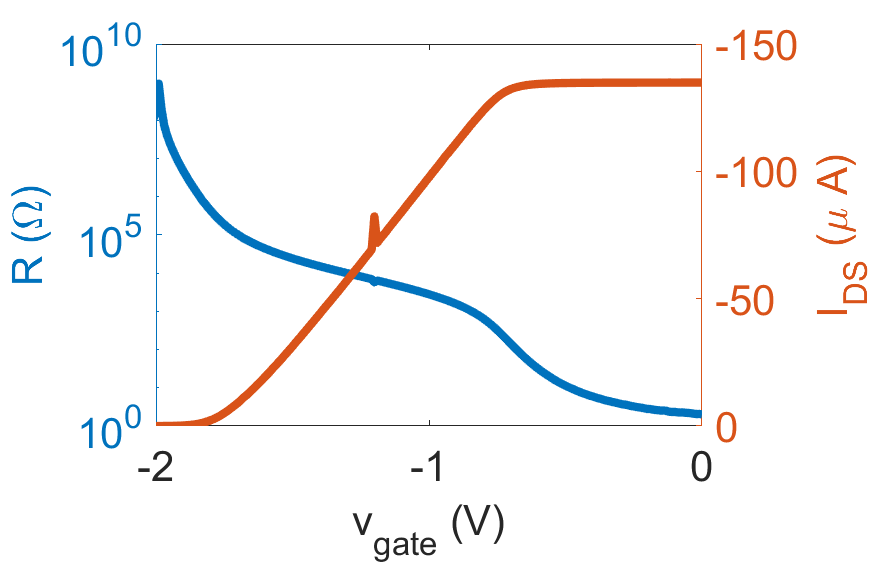
\includegraphics[width = 0.75\textwidth]{matlab_current_line.png}
    \caption{Current and resistance of the transistor as a function of gate voltage. Drain-source voltage is held constant at $v_{DS} = -1\si{\volt}$.}
    \label{fig:4wirecurrentline}
\end{figure}

\begin{figure} [H]
    \centering
    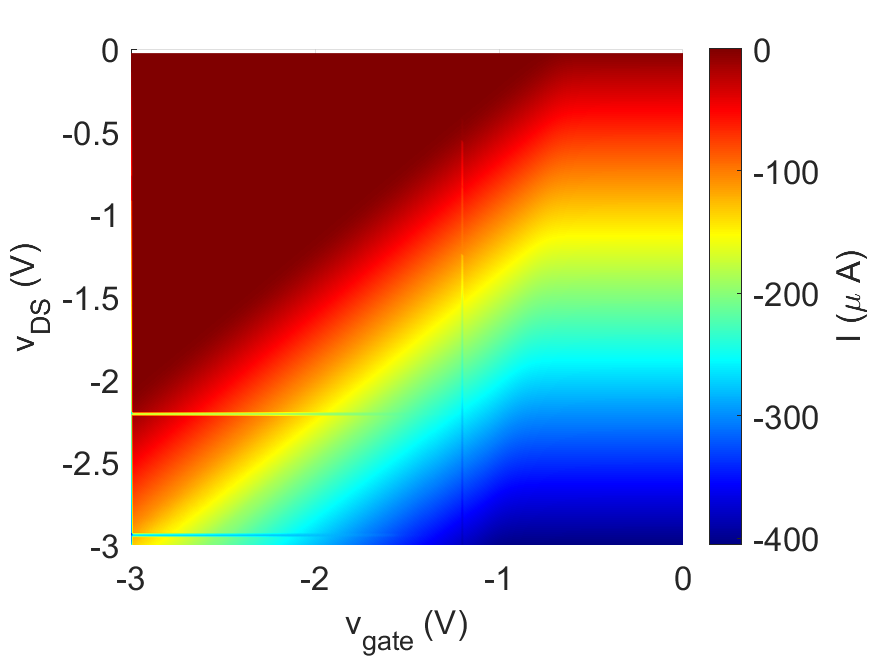
\includegraphics[width = 0.75\textwidth]{210208resistance_005_2021.02.10.17.23.31_final_i.png}
    \caption{Current through the transistor as a map of drain-source and gate voltages.}
    \label{fig:4wirecurrent}
\end{figure}
\begin{figure}[H]
    \centering
    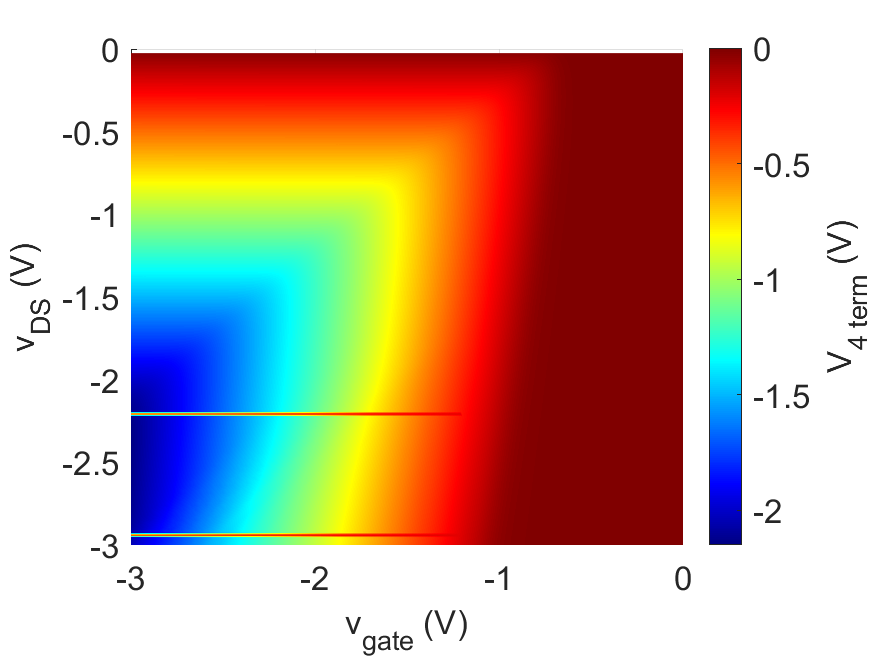
\includegraphics[width = 0.75\textwidth]{210208resistance_005_2021.02.10.17.23.31_final_v.png}
    \caption{Voltage of the transistor, using 4-wire sensing}
    \label{fig:4wirevoltage}
\end{figure}
\begin{figure}[H]
    \centering
    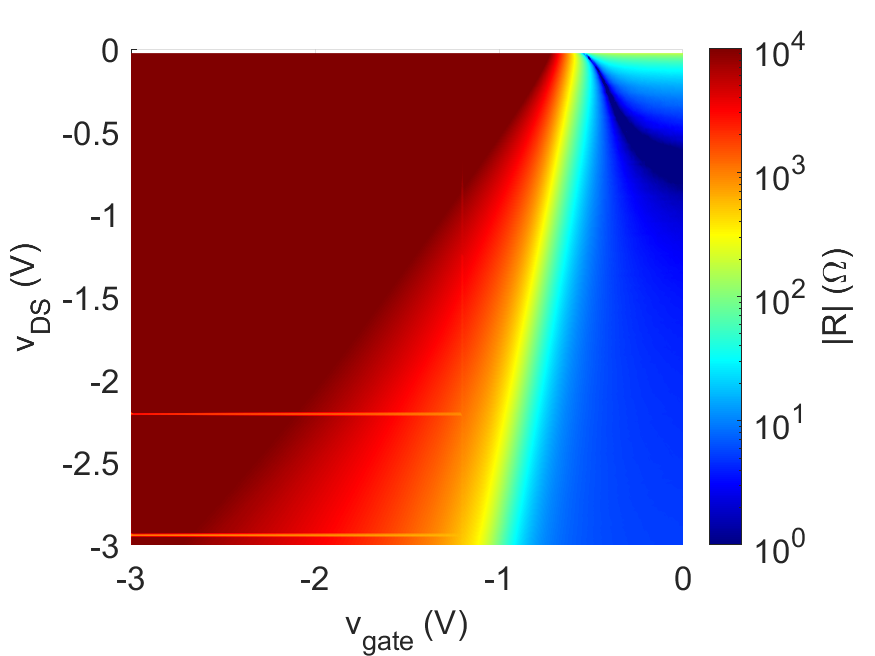
\includegraphics[width = 0.75\textwidth]{210208resistance_005_2021.02.10.17.23.31_final_res.png}
    \caption{Resistance of the transistor, using 4-wire sensing}
    \label{fig:4wireresistance}
\end{figure}

\begin{table}[H]
    \centering
    \begin{tabular}{| c | c  | c | c | c |}
        \hline
        Inductor & $f_\mathrm{res}$ (\si{\mega\hertz}) & $L$ (\si{\nano\henry}) & $C_p$ (\si{\pico\farad}) & Status \\[0.5ex]
        \hline \hline
        $L1$     & $164$                               & $1200$                 & $0.79$                   & -      \\
        $L2$     & $192$                               & $820$                  & $0.84$                   & -      \\
        $L3$     & $186$                               & $560$                  & $1.3$                    & Gate   \\
        $L4$     & $50$                                & $390$                  & $26$                     & Source \\ \hline
    \end{tabular}
    \caption{Measured resonant frequencies for each inductor on the Copenhagen board; Parasitic capacitance calculated using $f_\mathrm{res} = 1/2\pi\sqrt{LC_p}$.}
    \label{table:capacitances}
\end{table}

\begin{figure}[H]
    \centering
    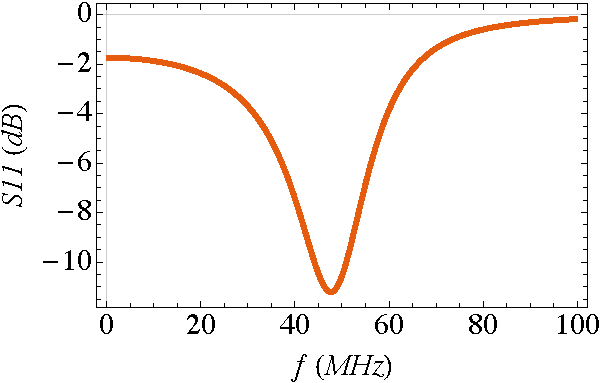
\includegraphics[width=0.7\textwidth]{S11_resonance.pdf}
    \caption{Simulated resonance peak at $R=1\si{\kilo\ohm}$ and $C_p = 26\si{\pico\farad}$. Resonance occurs at $f \approx 48\si{\mega\hertz}$.}
    \label{fig:resonancesim}
\end{figure}
\begin{figure}[H]
    \centering
    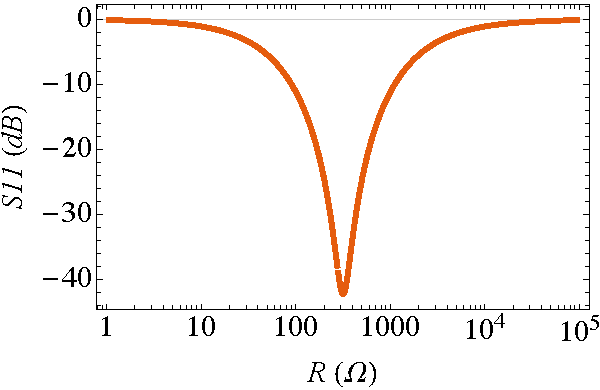
\includegraphics[width = 0.7\textwidth]{S11_cs0db.pdf}
    \caption{Simulated transfer function at resonant frequency.}
    \label{fig:s11cs0db}
\end{figure}

\begin{figure}[H]
    \centering
    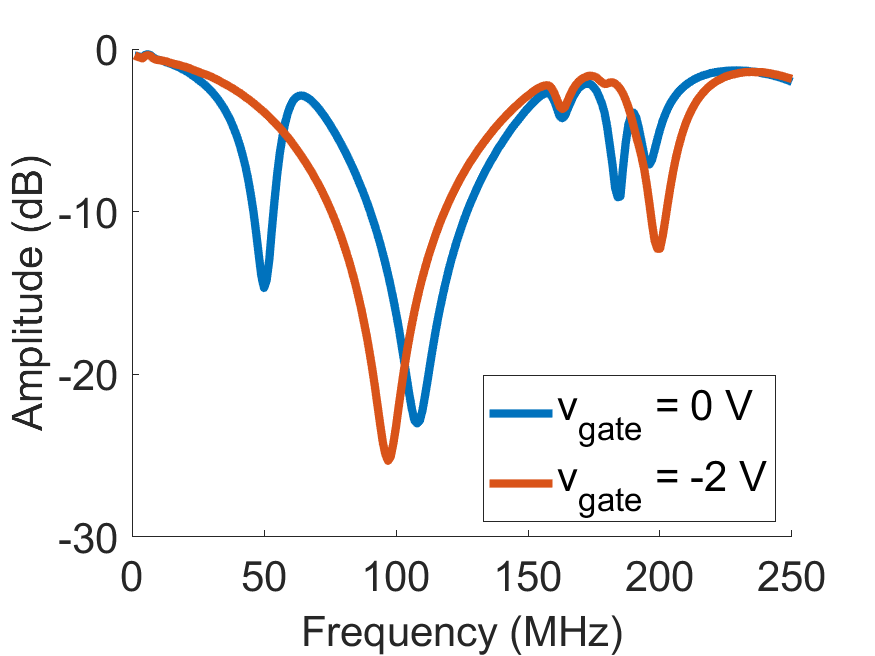
\includegraphics[width = 0.7\textwidth]{matlab_cs0_resonance.png}
    \caption{Resonance peaks at different gate voltages.}
    \label{fig:cs0res}
\end{figure}
\begin{figure}[H]
    \centering
    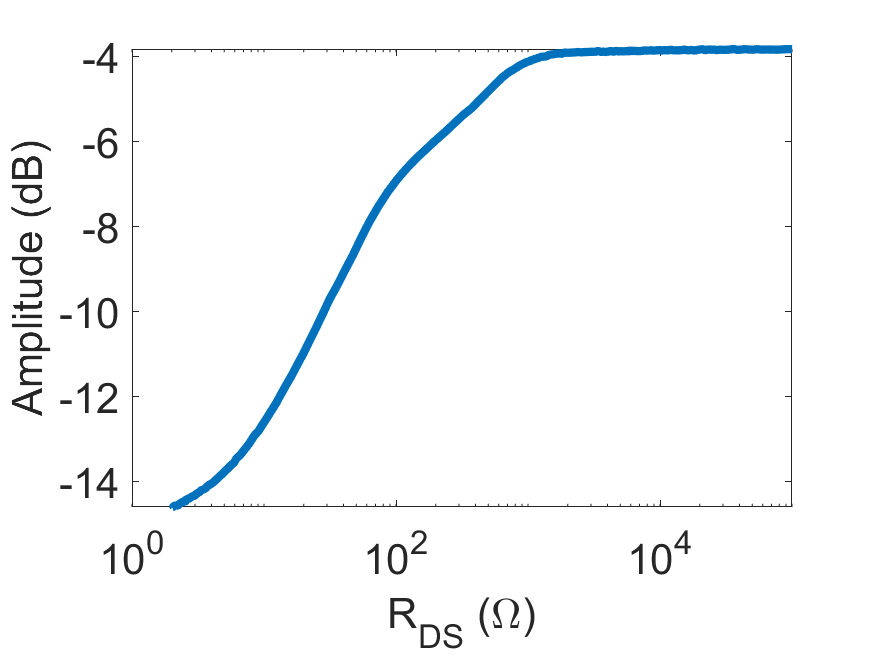
\includegraphics[width = 0.7\textwidth]{matlab_cs0_transfer.png}
    \caption{Transfer function at $f = 50\si{\mega\hertz}$ and $v_{DS} = -1\si{\volt}$.}
    \label{fig:cs0transfer}
\end{figure}

\begin{figure}[H]
    \centering
    \begin{circuitikz}[scale = 0.8]
        \draw
        (0,0) to[short, o-, i =$~$] (1,0) to[capacitor, l=$C_{BT}$] (2,0)
        to[capacitor, l=$C_9$] (3,0) to[capacitor, l=$C_6$] (4,0) -- (5,0)
        to[inductor, l=$L_4$] (6,0) -- (7,0) to[vR, l=$R$] (8,0) -- (9,0)
        to[capacitor, l=$C_{LF}$] (10,0) -- (10.5, 0) node[ground]{}
        % (4.5, 0) to[short, *-] (4.5, -2.5) to[C, l_=$C_s$] (5.5, -2.5) to[C, l_=$C_7$] (6.5, -2.5) -- (7, -2.5) node[ground]{}
        (6.5, 0) to[short, *-] (6.5, -1.5) to[C, l_=$C_p$] (7.5, -1.5) -- (8, -1.5) node[ground]{}
        ;
    \end{circuitikz}
    \caption{More accurate circuit diagram for the resonance circuit, with the transistor modelled as a variable resistor.}
    \label{fig:improvedcircuit}
\end{figure}

\begin{figure}[H]
    \centering
    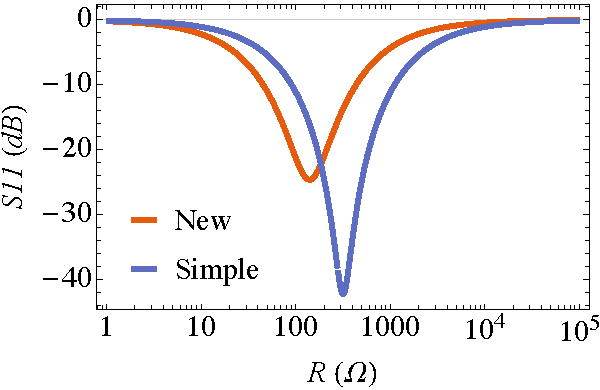
\includegraphics[width = 0.7\textwidth]{transfer_improved.pdf}
    \caption{Simulated transfer function comparison between the model from Figure \ref{fig:improvedcircuit} and that in the simple RLC circuit.}
    \label{fig:improvedtransfer}
\end{figure}

\begin{figure}[H]
    \centering
    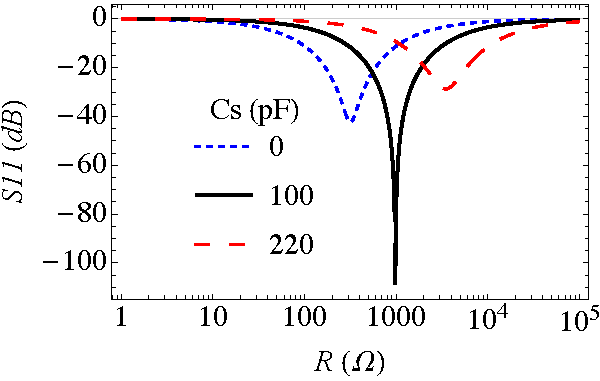
\includegraphics[width=0.7\textwidth]{cs_comparison.pdf}
    \caption{Comparison of transfer functions with shunt capacitors.}
    \label{fig:cscomparison}
\end{figure}

\begin{figure}[H]
    \centering
    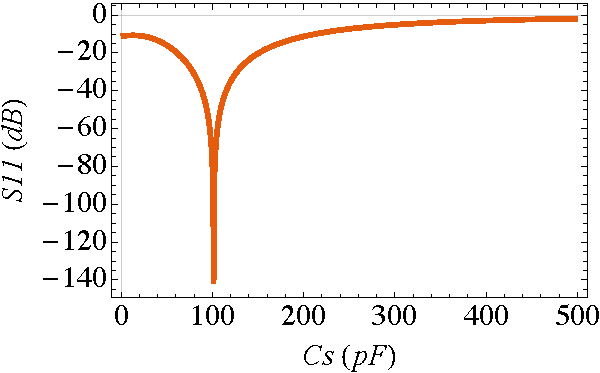
\includegraphics[width = 0.7\textwidth]{cs_simulation.pdf}
    \caption{Simulation of S11 values as a function of the included shunt capacitance, at a fixed value of $R = 1\si{\kilo\ohm}$.}
    \label{fig:cssimulation}
\end{figure}

\begin{figure}[H]
    \centering
    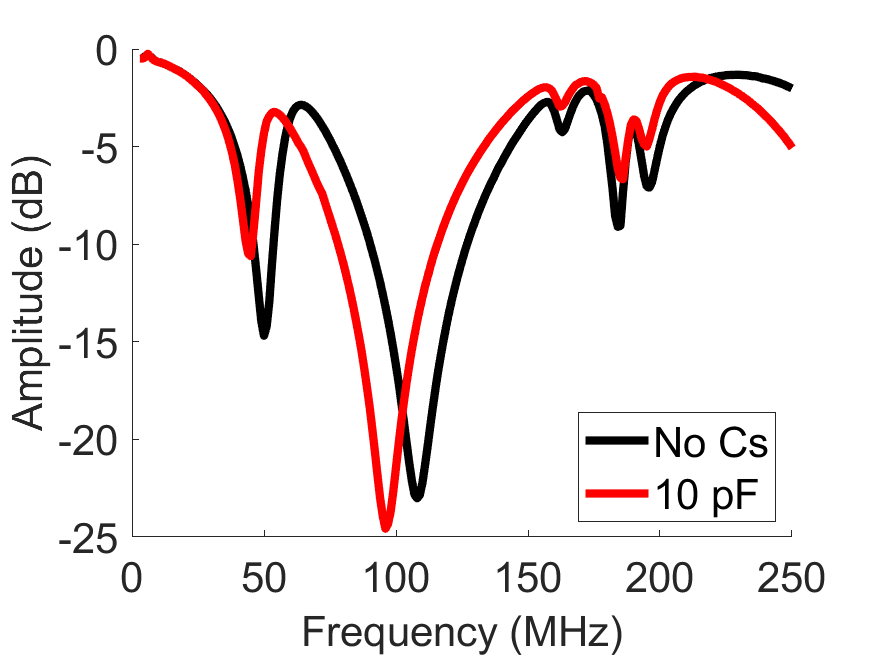
\includegraphics[width = 0.7\textwidth]{matlab_cs10_resonance.png}
    \caption{Resonance peaks with $C_s = 10\si{\pico\farad}$ and $C_s = 0$, holding $v_{DS} = -1\si{\volt}$, $v_\mathrm{gate}=0$.}
    \label{fig:cs10res}
\end{figure}
\begin{figure}[H]
    \centering
    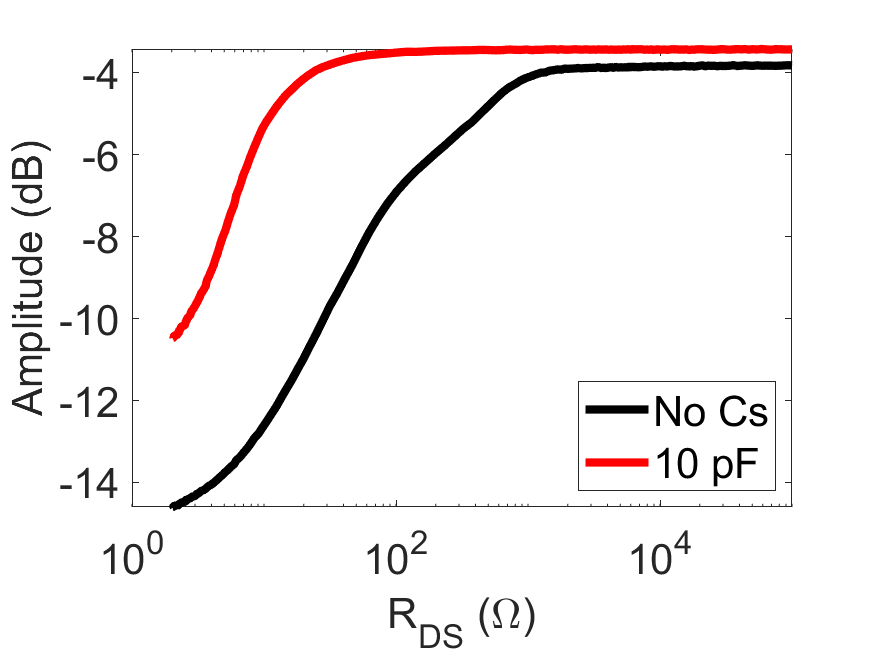
\includegraphics[width = 0.7\textwidth]{matlab_cs10_transfer.png}
    \caption{Transfer function at $f = 44\si{\mega\hertz}$ with $C_s = 10\si{\pico\farad}$ and at $f=50\si{\mega\hertz}$ with $C_s = 0$.}
    \label{fig:cs10transfer}
\end{figure}

\begin{figure}[H]
    \centering
    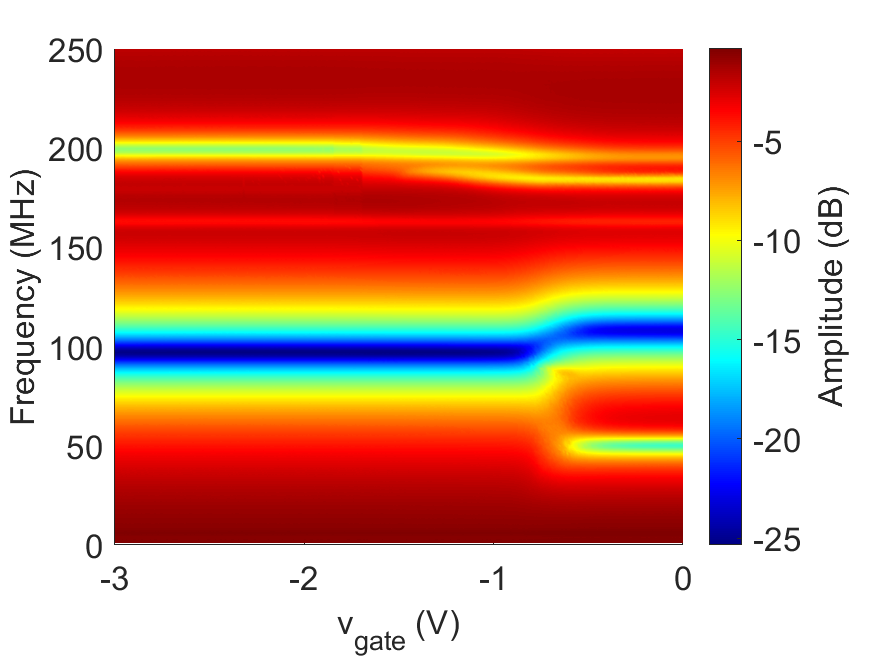
\includegraphics[width = 0.7\textwidth]{2102xxrf_001_2021.02.02.17.34.26_final_rf-surf.png}
    \caption{Resonance peaks at various $v_\mathrm{gate}$, without a shunt capacitor.}
    \label{fig:extra1}
\end{figure}
\begin{figure}[H]
    \centering
    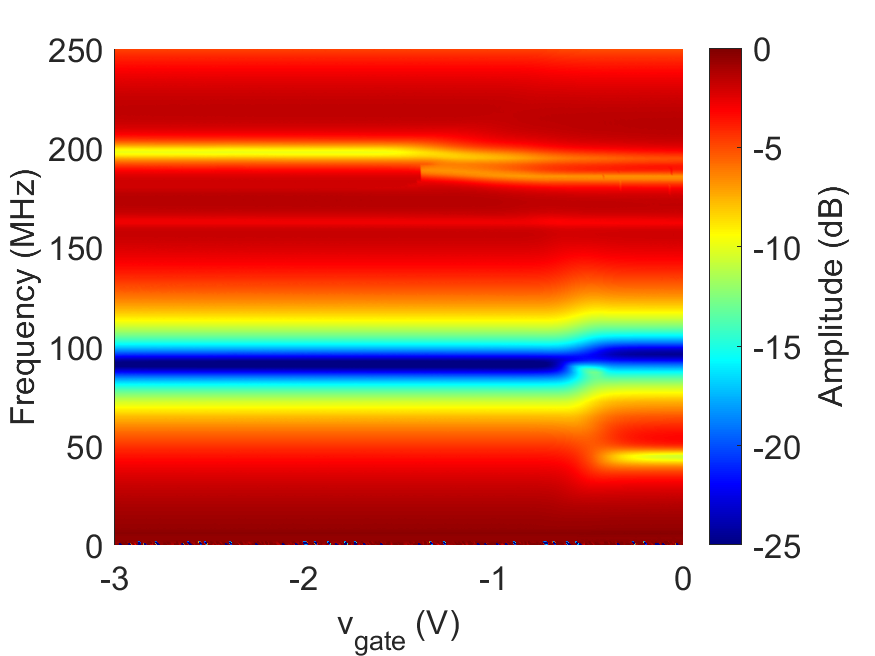
\includegraphics[width = 0.7\textwidth]{210212rf_003_2021.02.12.12.49.25_final_rf.png}
    \caption{Resonance peaks at various $v_\mathrm{gate}$, with $C_s = 10\si{\pico\farad}$.}
    \label{fig:extra2}
\end{figure}

\begin{figure}[H]
    \centering
    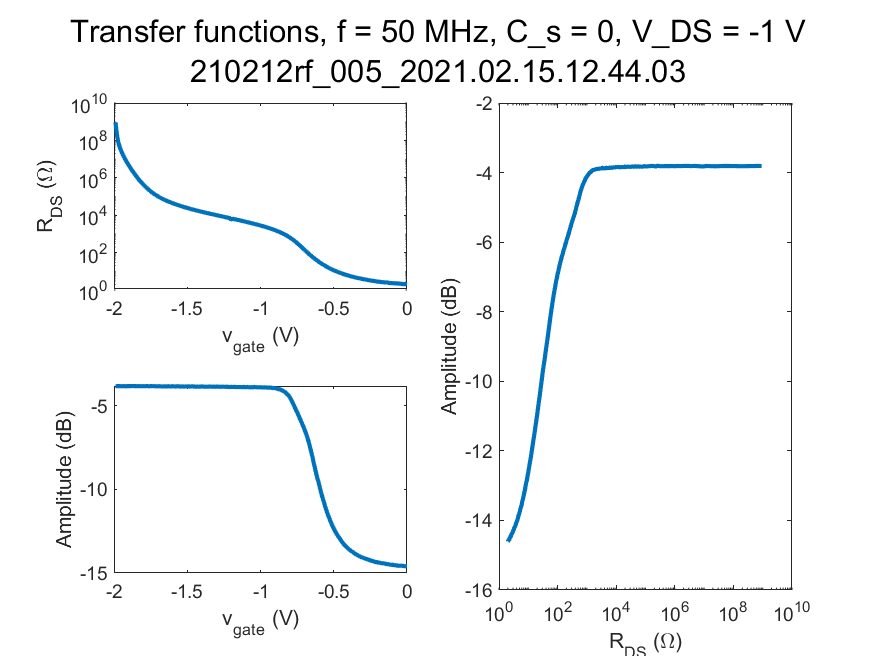
\includegraphics[width = 0.7\textwidth]{210212rf_005_2021.02.15.12.44.03_final_rf-transfer.png}
    \caption{Transfer function at $f = 50\si{\mega\hertz}$ and $v_{DS} = -1\si{\volt}$, with no shunt capacitor}
    \label{fig:extra3}
\end{figure}
\begin{figure}[H]
    \centering
    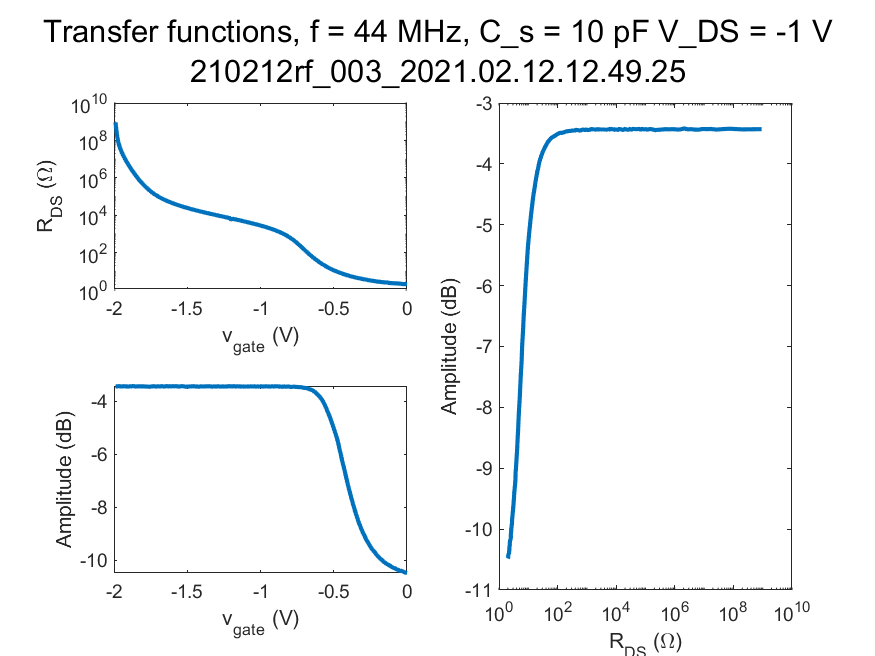
\includegraphics[width = 0.7\textwidth]{210212rf_003_2021.02.12.12.49.25_final_rf-transfer.png}
    \caption{Transfer function at $f = 44\si{\mega\hertz}$, with $C_s = 10\si{\pico\farad}$.}
    \label{fig:extra4}
\end{figure}

\begin{figure}
    \centering
    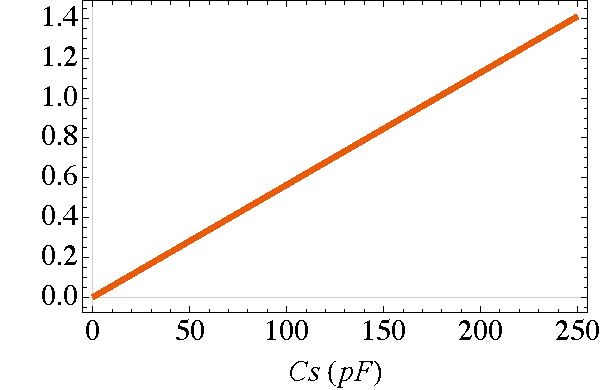
\includegraphics[width=0.7\textwidth]{impedanceratio.pdf}
    \caption{Ratio of RLC impedance to $C_s$ impedance as a function of $C_s$, at $f=50\si{\mega\hertz}$.}
    \label{fig:impedanceratio}
\end{figure}

\end{document}